


\documentclass{article}

% Language setting
% Replace `english' with e.g. `spanish' to change the document language

\usepackage{booktabs}
\usepackage{tabularx}
\usepackage{colortbl}
\usepackage{multirow}

\usepackage{bigstrut}
\usepackage{lipsum}

\usepackage{pifont}
% Set page size and margins
% Replace `letterpaper' with `a4paper' for UK/EU standard size
\usepackage[letterpaper,top=2cm,bottom=2cm,left=3cm,right=3cm,marginparwidth=1.75cm]{geometry}

% Useful packages
\usepackage{amsmath}
\usepackage{graphicx}
\usepackage[colorlinks=true, allcolors=blue]{hyperref}
\usepackage{cleveref}
\usepackage[english]{babel}
\usepackage{enumitem}


\usepackage{tikz}

\newcommand{\pie}[1]{%
\begin{tikzpicture}
 \draw (0,0) circle (0.5ex);\fill (0.5ex,0) arc (0:#1:0.5ex) -- (0,0) -- cycle;
\end{tikzpicture}%
}

\usepackage{pgfgantt}
\usepackage[
    backend=biber,
    style=ieee,
    maxbibnames=99,
    minbibnames=3,
    maxcitenames=2,
    mincitenames=1,
    citestyle=numeric-comp,
    sorting=none,
    dashed=false
]{biblatex}  
\title{PhD Midterm Report}
\author{Andr\'e Storhaug}

\addbibresource{refs.bib}

\begin{document}
\maketitle


\tableofcontents

%\begin{abstract}
%Your abstract.
%\end{abstract}

\section{Introduction}


\section{Project}

\subsection{Problem Statement}
In recent years, the field of language modeling has taken a huge leap in general language understanding. Large-scale transformer models \cite{vaswani2017attention} have shown great potential for general language understanding, surpassing almost every state-of-the-art language modeling task. This is especially due to the transformer's outstanding capability of transfer learning. Enormous amounts of resources are spent on pre-training transformer models on general knowledge. These models can then be fine-tuned for more specific tasks, building upon the already pre-trained knowledge.

Automatic code generation is by many considered the "holy grail" in the field of computer science \cite{PGL-010}. Recent works have applied transformers for code generation and program synthesis, achieving state-of-the-art results. For example, Codex by \textcite{chen2021codex} fine-tunes GPT-3 \cite{brown2020language} on code data from GitHub. Google DeepMind's AlphaCode by \textcite{li2022competition} trained an encoder-decoder model on code data from GitHub and fine-tuned it for competitive programming challenges.

Still, many challenges remain. One area of interest is the computational resources required for training the models. To update the model on new data, one often has to redo the entire fine-tuning process, an extremely resource-demanding process. Another problem is model bias. Due to the extensive data requirements for training these large models, the models often exhibit a lot of bias \cite{chen2021codex}. This could be everything from offensive language to vulnerable code.

The area of code synthesis with large language models is still in its early days. Especially interesting is the generation of smart contracts, which is the source code of blockchain applications. Although tricky to get right, smart contracts are often rather small and self-contained, making them a good candidate for automatic code generation. Some attempts have been made at summarizing smart contract code with large language models \cite{yang2021multimodal}. However, none have attempted the opposite, to automatically generate the smart contract code. This is what I have addressed in my master's thesis, in addition to investigating how to avoid introducing security vulnerabilities in the generated smart contract code. The doctoral thesis will be a continuation of my work, further investigating topics that would make the creation of smart contracts more available to people without expert knowledge, while simultaneously ensuring the generated code keeps high quality, is maintainable, and secure.

\subsection{Research Motivation}

However, besides bringing enhanced efficiencey, there is a lack of quality. The main motivation is to enable these automatic code generation systems to produce maintainable, secure, and correct code.


\begin{figure}[htbp]
    \centering
    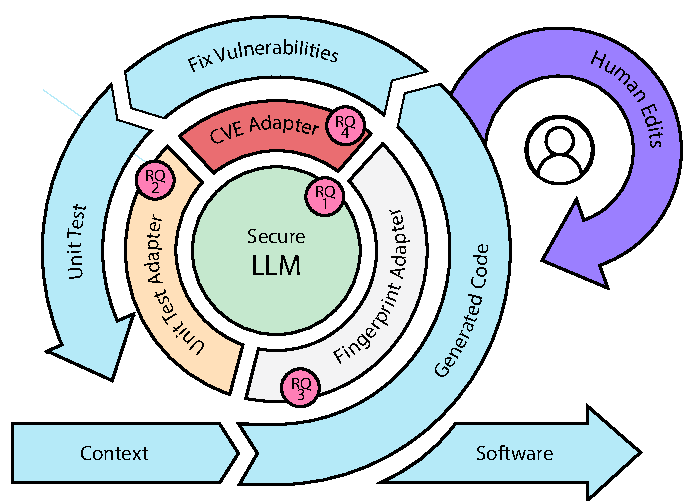
\includegraphics{figures/code_generation_lifecycle.pdf}
    \caption{Towards a holistic code generation framework.}
\end{figure}

\subsection{Research Questions}
The thesis aims to address the research motivations by answering the research questions for the thesis.

The overarching goal of the thesis is to figure out \textit{How to generate code that keeps high quality, is maintainable, and secure, using Large language models?}. This problem is broken down into five research questions. They are as follows:

\begin{enumerate}[leftmargin=2cm,label=\textbf{RQ\arabic*}:]
    \item How to automatically generate secure code with large language models?
    \item How to automatically generate unit tests?
    \item How to automatically generate integration tests?
    \item How to automatically fix code vulnerabilities introduced by humans?
\end{enumerate}


\begin{figure}[htbp]
    \centering
    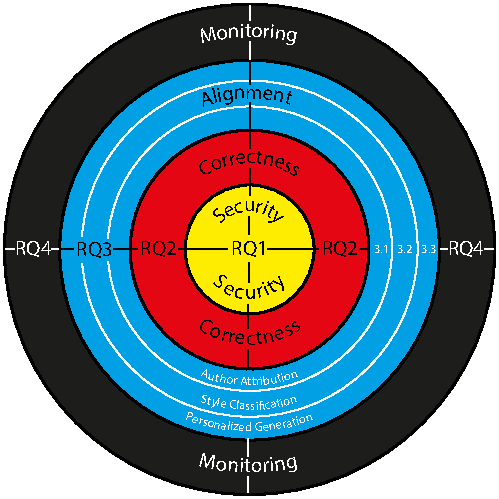
\includegraphics{figures/research_questions_bullseye.pdf}
    \caption{Research questions objectives and relation.}
\end{figure}

\subsection{Research Outcomes}


\subsubsection{Research Contributions}

\begin{enumerate}[leftmargin=2cm,label=\textbf{C\arabic*}:]
    \item \textit{New method for generating safe code with LLMs.} How to automatically generate secure code with large language models?
    \item \textit{New knowledge about how PEFT can be used for enhancing unit test generation.} How to automatically generate unit tests?
    \item \textit{New knowledge about how LLMs for code are able to adhere to the existing style.} How to align large language models with a developer's style, or ``fingerprint''.
    \item How to align large language models with a developer's style, or ``fingerprint''.
    \item How to automatically fix code vulnerabilities introduced by humans?
\end{enumerate}


\begin{table}[htp]
    \newcolumntype{Y}{>{\centering\arraybackslash}X}
    \centering
    \caption{Relationship between publications, research questions (RQs) and contributions.}
    \label{tab:my_label}
    
    \begin{tabularx}{\textwidth}{l|YYYY|YYYY}
        \toprule
         & \multicolumn{4}{c}{\textbf{Research Questions}} & \multicolumn{4}{c}{\textbf{Contributions}}\\
         \textbf{Papers} & RQ1 & RQ2 & RQ3 & RQ4 & C1 & C2 & C3 & C4\\
        \midrule
        Paper A - Vulnerability-constrained decoding & \bullet & & & & \bullet & & & \\
        Paper B - Unit Test Generation & & \bullet & & & & \bullet & & \\
        Paper C - Source Code Author Attribution & & & \bullet & & & & \bullet & \\
        Paper D - Can LLMs follow code style? & & & \bullet & & & & \bullet & \\
        Paper E - Aligning LLMs to code fingerprints & & & \bullet & & & & \bullet & \\
        Paper F - Automatic fixing of code vulnerabilities & & & & \bullet & & & & \bullet\\
        \bottomrule
    \end{tabularx}
\end{table}

\begin{table}[htp]
    \newcolumntype{Y}{>{\centering\arraybackslash}X}
    \centering
    \small
    \caption{Dissemenation Plan}
    \label{tab:my_label}
    
    \begin{tabularx}{\textwidth}{cp{5cm}XlXX}
        \toprule
        \textbf{ID} & \textbf{Title} & \textbf{Publisher} & \textbf{Conference} & \textbf{Method} & \textbf{Status} \\
        \midrule
        A & Efficient Avoidance of Vulnerabilities in Auto-completed Smart Contract Code Using Vulnerability-constrained Decoding & IEEE & ISSRE 2023 \cite{issre} & Design Science \cite{ralph2021empirical} & Published \\
        B & Parameter-Efficient Fine-Tuning of Large Language Models for
Unit Test Generation: An Empirical Study & IEEE/ACM & ASE 2024 \cite{ase} & Benchmarking \cite{ralph2021empirical} & Submitted \\
        C & Source Code Authorship Attribution Using Large Language Models & IEEE/ACM & ICSE 2025 \cite{icse} & Design Science \cite{ralph2021empirical} &  \\
        D & Can LLMs follow code style? & ??? & ??? \cite{icse} &   Exploratory Data Science \cite{ralph2021empirical}& ??? \\
        E & Aligning LLMs to code fingerprints & ??? & ??? & ???\\
        F & Automatic fixing of code vulnerabilities & ??? & ??? & ???\\
        \bottomrule
    \end{tabularx}
\end{table}

contrib
new method for generating secure code

Knowledge on test generation peft


We propose a novel vulnerability-constrained decoding approach to avoid vulnerabilities in the generated code efficiently and effectively. The approach can help com- panies quickly update LLMs to avoid the negative con- sequence caused by vulnerabilities in the model training dataset.

We conducted the first empirical study to extensively eval-
uate training LLMs using various PEFT methods—LoRA,
(IA)3, and prompt tuning—for unit test generation across a
wide range of LLM models

\subsection{Paper A - Secure code generation}

\textbf{Efficient Avoidance of Vulnerabilities in Auto-completed Smart Contract Code Using Vulnerability-constrained Decoding}\\\\
\noindent Andr\'e Storhaug, Jingyue Li, Tianyuan Hu\\\\
\noindent \textbf{Published in}: 2023 IEEE 34th International Symposium on Software Reliability Engineering (ISSRE), Florence, Italy, 2023, pp. 683-693, doi: 10.1109/ISSRE59848.2023.00035.\\\\
\noindent \textbf{Research Question}: RQ1\\\\
\noindent \textbf{Main Area of Contribution}: \\\\

Masters use only $$<|secure|> and <|vulnerable|>$$ labels. Vulnerability constrained decoding builds upon initial work done in master thesis. the approach is refined and greatly improved. Uses actually vulnerability types. Named vulnerability constraned decoding.

For my master thesis, I have studied how to automatically generate secure smart contract code for the Ethereum blockchain. The code generation was done by fine-tuning a 6-billion parameter large transformer model (GPT-J \cite{gpt-j}) on a smart contract dataset consisting of 53 million lines of code. Contributions include the currently largest smart contract dataset, and a state-of-the-art automatic smart contract code generation model. In addition, the project tackles the problem of dataset bias, focusing on reducing security vulnerabilities that are introduced by these large-scale datasets. Using the code generator developed in my thesis, smart contract code developers can generate secure smart contract code by only writing comments to describe the functions to be provided by the code. The results and findings from my master thesis can be further analyzed and the approach refined in my PhD studies.

\subsection{Paper B - Unit Test Generation using PEFT}
\textbf{Parameter-Efficient Fine-Tuning of Large Language Models for Unit Test Generation: An Empirical Study}\\\\
\noindent Andr\'e Storhaug, Jingyue Li\\\\
\noindent \textbf{Research Question}: RQ2\\\\
\noindent \textbf{Main Area of Contribution}: \\\\

How to efficiently update the AI-model for providing up-to-date high-quality code?
Software development is an ever-evolving industry. Code libraries are updated, new vulnerabilities are discovered, APIs are changed, etc. As a developer, one of the primary skills is to be able to quickly adapt to such changes. For automatic code generation systems to be on par with humans, these systems must be also able to produce up-to-date high-quality code. However, training large transformer models normally entails an extremely high resource consumption. Investigating methods for efficient retraining and adaptations are therefore highly relevant. For example, in the area of smart contracts, a vast number of contracts are made available each day. By additively continuing training of large-scale transformer models in an energy-efficient way, one could ensure the model provides up-to-date high-quality code.

\subsection{Paper C - Source Code Author Attribution}

\textbf{Source Code Authorship Attribution Using Large Language Models}\\\\
\noindent Andr\'e Storhaug, Jingyue Li\\\\
\noindent \textbf{Research Question}: RQ3.1\\\\
\noindent \textbf{Main Area of Contribution}: \\\\

Another problem rooted in model bias is the issue of producing maintainable code. Due to the share volume of data needed for training large-scale transformer models, freely available code hosted on platforms such as GitHub is normally used for pre-training. A lot of the data available on such platforms are not maintainable, contains ad hoc solutions and has a bad coding style. This will inevitably affect the quality of the model's generated code. For automatic code generation to be used in a production setting, the generated code needs to be maintainable and understandable so that developers can integrate the manually developed code and the auto-generated code. Investigating methods for combating code smells, would massively improve the usefulness of such an automated system.

\subsection{Paper D - Code Style Classification}

\textbf{Can LLMs follow code style?}\\\\
\noindent Andr\'e Storhaug, Jingyue Li\\\\
\noindent \textbf{Research Question}: RQ3.2\\\\
\noindent \textbf{Main Area of Contribution}: \\\\

Another problem rooted in model bias is the issue of producing maintainable code. Due to the share volume of data needed for training large-scale transformer models, freely available code hosted on platforms such as GitHub is normally used for pre-training. A lot of the data available on such platforms are not maintainable, contains ad hoc solutions and has a bad coding style. This will inevitably affect the quality of the model's generated code. For automatic code generation to be used in a production setting, the generated code needs to be maintainable and understandable so that developers can integrate the manually developed code and the auto-generated code. Investigating methods for combating code smells, would massively improve the usefulness of such an automated system.



\subsection{Paper D - Personalized Code Generation?}

\textbf{Aligning LLMs to code fingerprints}\\\\
\noindent Andr\'e Storhaug, Jingyue Li\\\\
\noindent \textbf{Research Question}: RQ3.3\\\\
\noindent \textbf{Main Area of Contribution}: \\\\

Automatic code generation could help developers produce more secure, maintainable, and high-quality code at a fast pace. By further combining graphical tools like VPL \footnote{Microsoft Visual Programming Language (VPL) \url{https://docs.microsoft.com/en-us/previous-versions/microsoft-robotics/bb483088(v=msdn.10)}} with automatic code generation, one could extend a lot of these benefits to users beyond the standard developer.  No-code solutions are increasing in popularity, however, most of these systems are still rooted in standard code generation techniques. By leveraging the capabilities of large-scale language models, one could significantly enhance and simplify how the user interacts with such systems. It could open up new and more flexible ways for how programs are created. Not only would this greatly lower the threshold for non-developers to leverage programming, but also increased efficiency due to a simpler developing process.


\subsection{Paper E - Security fixing?}

\textbf{Automatic fixing of code vulnerabilities}\\\\
\noindent Andr\'e Storhaug, Jingyue Li, Jiamou Sun, Jieshan Chen, Zhenchang Xing\\\\
\noindent \textbf{Research Question}: RQ3.3\\\\
\noindent \textbf{Main Area of Contribution}: \\\\



\section{Academic Training}

\subsection{Plan for Completion}
\lipsum[1-2]
\begin{figure}[htpb]
%\thispagestyle{empty}
%\begin{landscape}
	\clearpage
	%\newgeometry{margin=2.5cm, top=20mm, bottom=35mm}
\definecolor{foobarblue}{RGB}{0,153,255}

\newganttchartelement{mainbar}{
    mainbar/.style={
        draw=foobarblue!10!black,
        fill=foobarblue!10
    },
    mainbar label font=\bfseries
}

\newganttlinktype{f-m}{
 \ganttsetstartanchor{on right=1}
 \ganttsetendanchor{on left=0}
 \draw[/pgfgantt/link]
  ([xshift=-.2pt]\xLeft, \yUpper) -- 
  (\xRight, \yLower);
}

\hspace{-2cm}
\noindent
\begin{ganttchart}[
    progress=today,
    today=25,
    today label=August,
    hgrid,
    vgrid={*{2}{draw=none},{dotted}},
    vrule label font=\tiny,         
    title label font=\tiny,
    %bar label font=\tiny,
    %milestone label font=\tiny,
    %group label font=\bfseries\small,
    bar height = 0.4,
    %milestone left shift =-1,
    %milestone right shift =1,
    x unit=0.325cm,
    y unit title=.6cm,
    %y unit chart=0.85cm,
    y unit chart=0.7cm,
    link bulge = 2,
    bar label node/.append style={align=left},
    link/.style={-latex, draw=red, fill=red, thick}
    ]{1}{42}
    %labels
    \gantttitle[]{2022}{6}                 % title 2
    \gantttitle[]{2023}{12}
    \gantttitle[]{2024}{12}
    \gantttitle[]{2025}{12}\\
    \gantttitlelist{"Q3","Q4"}{3}
    \gantttitlelist{"Q1","Q2","Q3","Q4"}{3}
    \gantttitlelist{"Q1","Q2","Q3","Q4"}{3}
    \gantttitlelist{"Q1","Q2","Q3","Q4"}{3}\\
    %tasks
    \ganttgroup{Organised academic training}{2}{30} \\
    \ganttbar{Corse IDT8000}{2}{6} \\
    \ganttbar{Corse IDT80002}{2}{6} \\
    \ganttbar{Corse DT8111}{7}{12} \\
    \ganttbar{Corse DT8806}{7}{12} \\
    \ganttbar{FYS-8805 (Winter school)}{7}{7} \\
    \ganttbar{Corse DT8114}{25}{30} \\
    
    \ganttgroup{Research}{2}{34} \\
    \ganttset{ bar/.append style={fill=yellow}, bar incomplete/.append style={fill=yellow!10}}%
    \ganttbar[name=RQ1]{RQ1}{2}{12} \\
    \ganttmilestone[name=M1]{Paper to ISSRE 2023}{12} \\
    \ganttset{ bar/.append style={fill=red}, bar incomplete/.append style={fill=red!10}}%
    \ganttbar[name=RQ2]{RQ2}{13}{24} \\
    \ganttmilestone[name=M2]{Paper to ASE 2024}{24} \\
    %\ganttbar[name=RQ3]{RQ3}{24}{25} \\%6+12+7 /juni
    \ganttset{ bar/.append style={fill=blue}, bar incomplete/.append style={fill=blue!10}}%
    \ganttbar[name=RQ31]{RQ3.1}{24}{26}\\ %6+12+7 /juni
    \ganttmilestone[name=M31, milestone label node/.append style={align=right}]{Paper to ICSE 2025}{26}\\
    \ganttbar[name=RQ32]{RQ3.2}{27}{28} \\
    \ganttmilestone[name=M32, milestone label node/.append style={align=right}]{Paper to JSS 2025}{28}\\
    \ganttbar[name=RQ33]{RQ3.3}{29}{34} \\
    \ganttmilestone[name=M33, milestone label node/.append style={align=right}]{Paper to TSE 2025}{34}\\
    %\ganttmilestone{}{29}
    %\ganttmilestone{}{25}\\
    \ganttgroup[group label node/.append style={align=right}]{Exchange to CSIRO's Data61}{27}{32}\\
    \ganttset{ bar/.append style={fill=black}, bar incomplete/.append style={fill=black!50}}%
    \ganttbar[name=RQ4]{RQ4}{27}{32} \\
    \ganttmilestone[name=M4]{Paper to ?}{32} \\
    \ganttbar[name=T1]{\textbf{Thesis writing}}{35}{39} \\
    \ganttmilestone[name=W1, milestone label node/.append style={align=right}]{Deliver thesis}{39}
    % 
    \ganttlink[link type=f-m]{RQ1}{M1}
    \ganttlink[link type=f-m]{RQ2}{M2}
    \ganttlink[link type=f-m]{RQ31}{M31}
    \ganttlink[link type=f-m]{M31}{RQ32}
    \ganttlink[link type=f-m]{RQ32}{M32}
    \ganttlink[link type=f-m]{M32}{RQ33}
    \ganttlink[link type=f-m]{RQ33}{M33}
    \ganttlink[link type=f-m]{RQ4}{M4}
    \ganttlink[link type=f-m]{T1}{W1}
    %\ganttlink{RQ2}{RQ3}
    %\ganttlink{RQ3}{RQ4}
    %\ganttlink{RQ4}{W1}
\end{ganttchart}
%\restoregeometry
	\caption{Gantt diagram of working plan.}
	\label{fig:gantt-diagram-progress-plan}
\end{figure}


\subsection{Changes in Academic Content}


\subsection{Organised Academic Training}


\begin{table}[htp]
    \newcommand\T{\rule{0pt}{2.6ex}}       % Top strut
    \newcommand\B{\rule[-1.2ex]{0pt}{0pt}} % Bottom strut
    \centering
    \caption{Course plan status}
    \label{tab:my_label}
    
    \begin{tabularx}{\textwidth}{Xllcc}
        \toprule
        \textbf{Code} & \textbf{Title} & \textbf{Term} & \textbf{Level} & \textbf{ECTS}\\
        \midrule
        \multicolumn{5}{l}{\cellcolor{green!20}{\textbf{Completed}}} \bigstrut\\
        \T IDT8000 & Research Ethics & 2022 A & PhD & 2.5\\
        IDT8002 & Project development and management & 2022 A & PhD & 2.5\\
        DT8111 & Empirical research methodologies in ID and digitalization & 2023 S & PhD & 7.5\\
        DT8806 & ISSE Research Topics and Academic Writing & 2024 S & PhD & 7.5\\
        FYS-8805 & NLDL Deep Learning Winter School 2023 & 2023 S & PhD & 5\\
        \midrule
        \multicolumn{4}{l}{Total completed ETCS} & 25\\
        \midrule
        \midrule
        \multicolumn{5}{l}{\cellcolor{yellow!20}{\textbf{Planned}}} \bigstrut\\
        \T DT8114 & PhD Seminar in Computer and Information Science & 2023 S & PhD & 7.5\\
        \midrule
        \multicolumn{4}{l}{Total planned ETCS} & 7.5\\
        \midrule
        \bottomrule
    \end{tabularx}
\end{table}


\subsection{Academic services}

Every other week?

"Co-supervised" find name of previous student.
Co-supervisor for Petter Dahlen master thesis.

Web Co-host together with Alicia for FSE 2025.

\subsection{Community Engagement}

\begin{table}[htp]
    \newcommand\T{\rule{0pt}{2.6ex}}       % Top strut
    \newcommand\B{\rule[-1.2ex]{0pt}{0pt}} % Bottom strut
    \centering
    \caption{Course plan status}
    \label{tab:my_label}
    
    \begin{tabularx}{\textwidth}{lllXc}
        \toprule
        \textbf{Code} & \textbf{Title} & \textbf{Term} & \textbf{Level} & \textbf{ECTS}\\
        \midrule
        \multicolumn{5}{l}{\cellcolor{green!20}{\textbf{Completed}}} \bigstrut\\
        \T IDT8000 & Research Ethics & 2022 A & PhD & 2.5\\
        IDT8002 & Project development and management & 2022 A & PhD & 2.5\\
        
    \end{tabularx}
\end{table}

Winterschool Tromsø


NORAI conference

Workshop birgit (sustainability?)
ISSE seminar
Intensive course on scientific publishing
Blockheim 2024 - Trondheim Open Blockchain Meetup
Attended ICSE conference


\subsection{External Research Stay}



\section{Ethical reflections}
The very nature of machine learning models gives raise to several ethical issues. Firstly, these systems might be biased. If the dataset used for training is biased, the model might perpetuate social prejudices and injustices. Proper care should be taken to reduce the likelihood of producing biased models. Secondly, the systems might be used for evil. Automatic code generation can significantly increase productivity of developers. However, these systems may also help attackers write malicious code. It is therefore important to thoroughly assess these capabilities before releasing models to the general public, ensuring that the benefits outweigh the risks.

\section{Sustainability}
One of the more important UN goal is the 13th: climate action. Global warming is one of the most critical challenges the world is facing today. Large-scale transformer model requires a huge amount of training resources. Of special significance is the amount of electricity required to power the necessary computing platform. For example, the estimated carbon emissions due to training GPT-3, a 175 billion parameter transformer model, are 552 tonnes $CO_2$ and an energy consumption of 1287 MWh \cite{patterson2021carbon}. In my research, I will primarily aim to reuse (fine-tune) existing models, keeping both the environmental impact and costs as low as possible. Further, by making most of the results from this research open source, others may benefit from this work. By making both models and datasets available for other researchers and the general public, this will reduce the need for everyone creating their own solution, further reducing the required climate footprint. This is also naturally related to the 12th UN goal: responsible consumption and production. In relation to the ethical aspects of bias described in the previous section, this concerns both the 5th and 10th UN sustainability goals; Gender equality and Reduced inequalities.

\section{Conclusion}


%\bibliographystyle{ieee}
\vspace{1cm}
\newpage
\printbibliography
\end{document}



//. some comment
function helloworld(int number) retunr {

    print(98ifi
    }
    
    /comment
    
    
    
// print hello 
